\section {System Overview\\}

\subsection{Design Goals and Rationale\\}
The design of the PushUp server is driven by the following rationales.
\begin{itemize}
\item {\bf Large Concurrent Connections}:
    As the long polling technologies requires the server to keep the polling
    request active for a period of time, large number of concurrent clients 
    will generate lots of active connections. One of the most goal of PushUp
    is to minimize the cost of maintaining these active concurrent connections,
    which can in turn enhance the system's scalability.
     
    The key to reduce the cost is the event-based notification mechanism provided
    by the operating systems. Unlike the multi-process or multi-threading concurrent
    model, the event-based concurrency model requires much less resource to maintain
    the connections.
\item {\bf Transparency}: Although event-based concurrency significantly reduce the 
    maintenance cost, it is impractical to have all the web server to be implemented
    in event-based programming style. Rather, we hope the existing web servers can 
    have the efficient long polling with minimal modification.

    So when designing the PushUp server, much effort is made to ensure that 
    the web servers and clients can work with minimal awareness of PushUp 
    server's existence.
\item {\bf Low latency}: Adding an intermediate layer in between of the 
    clients and web servers will inevitably create some overhead. 
    The PushUp server should not create too much extra costs.

\item {\bf Generality}: The PushUp Server is designed for general purposes. It is
    not designed for a specific system for some specific purposes.

\end{itemize}

\subsection{System Overview\\}

TODO: a figure to illustrate the main idea.

\begin{figure}[htb!]
\centering%
    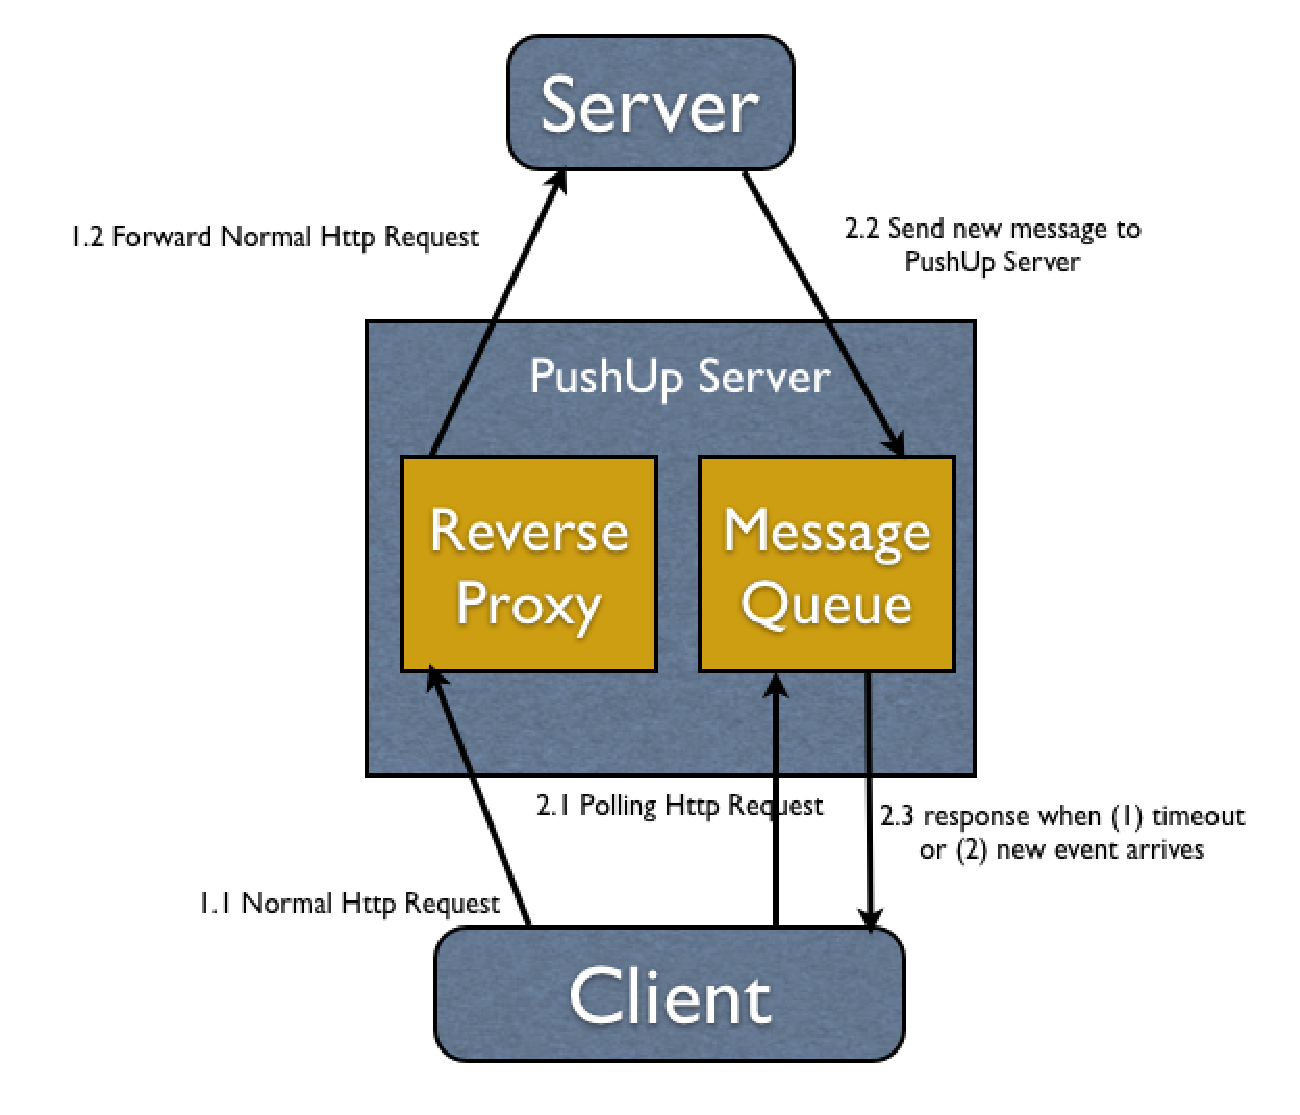
\includegraphics[scale=0.40]{figures/simple_pushup_arch.eps}
    \caption{Simplified PushUp Architecture}
    \label{fig:eventloop}
\end{figure}

TODO: Overall description of such design. and how it matches the rationale mentioned above.


\subsection{Reverse Proxy\\}

Why reverse proxy

How it works. Briefly

\subsection{Message Queue\\}

Why Message Queue, 

How it works, briefly


